\begin{pastexam}[label={px:gw3-099-ds-04}]{關務三等資訊處理 99 年 第五題}
（申論；20 分）

拓樸排序（topological sorting）是一個在沒有迴圈的有向性圖形（directed graph）找出節點順序（Linear order）。
例如，如果有一條有向連結從節點 u 指向節點 v，則我們說 u v 的順序為 u 在 v 的前面。拓樸排序的演算法如下：
\begin{quote}
topSort（input Graph, output List）\\
\hspace*{1em}s=createStack();\\
\hspace*{1em}for (all vertices v in the graph)\\
\hspace*{3em}if (v has no predecessors) \{\\
\hspace*{4em}Push v into s;\\
\hspace*{4em}Mark v as visited;\}\\
\hspace*{1em}while (s is not empty) \{\\
\hspace*{3em}if (all vertices adjacent to the vertex v on the top of the stack have\\
\hspace*{5em}been visited) \{\\
\hspace*{7em}Pop v out of s;\\
\hspace*{7em}Output v;\\
\hspace*{3em}\} else \{\\
\hspace*{7em}Push each unvisited vertex u adjacent to vertex v into s and\\
\hspace*{7em}mark u as visited; // 注意：當有一個以上的選擇時，永遠\\
\hspace*{7em}優先選擇代號數字比較小的節點先放入堆疊\\
\hspace*{4em}\}\\
\hspace*{1em}\}
\end{quote}
\begin{enumerate}[leftmargin=2.2em]
\item[㈠] 以下為一個有向性圖形，請利用以上程式列出所找出的節點順序。（請列出執行過程堆疊（stack）內的內容）
（10 分）
\begin{center}
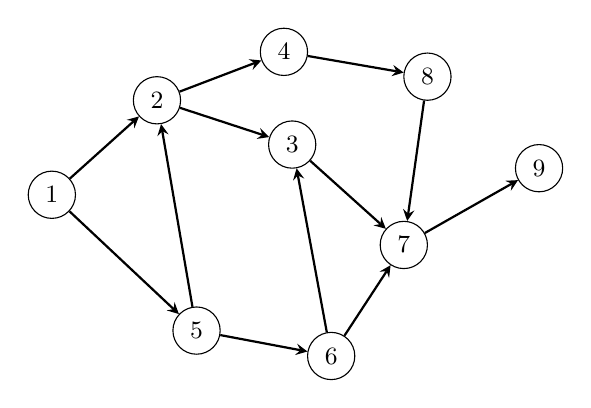
\begin{tikzpicture}[x=0.75cm, y=0.75cm, >=stealth,
    v/.style={circle, draw, minimum size=6mm, inner sep=0pt, font=\small}]
\node[v] (1) at (0.4,-2.6) {1};
\node[v] (2) at (2.18,-1.0) {2};
\node[v] (4) at (4.33,-0.18) {4};
\node[v] (8) at (6.76,-0.6) {8};
\node[v] (3) at (4.47,-1.75) {3};
\node[v] (9) at (8.65,-2.15) {9};
\node[v] (7) at (6.36,-3.45) {7};
\node[v] (5) at (2.85,-4.9) {5};
\node[v] (6) at (5.13,-5.33) {6};
\draw[->, thick] (1) -- (2);
\draw[->, thick] (1) -- (5);
\draw[->, thick] (5) -- (2);
\draw[->, thick] (2) -- (4);
\draw[->, thick] (2) -- (3);
\draw[->, thick] (4) -- (8);
\draw[->, thick] (8) -- (7);
\draw[->, thick] (3) -- (7);
\draw[->, thick] (5) -- (6);
\draw[->, thick] (6) -- (3);
\draw[->, thick] (6) -- (7);
\draw[->, thick] (7) -- (9);
\end{tikzpicture}
\end{center}
\item[㈡] 如果有向性圖 G=（V, E），節點集合的大小為 N，請問此演算法的時間複雜度（time complexity）Big-O
為何？（請說明如何得到答案）（10 分）
\end{enumerate}
\end{pastexam}

\begin{pastsoln}
圖的邊：1→2、1→5、5→2、2→3、2→4、4→8、8→7、3→7、5→6、6→3、6→7、7→9。 只有節點 1 沒有前驅
（入分支度為 0）。

\textbf{題意與原題的問題。} 「優先選擇代號數字比較小的節點先放入堆疊」照字面解讀：一次要 push 好幾個
節點時，編號小的先 push，所以編號大的在上面、會先被處理。 這個演算法是用堆疊模擬 DFS：一個節點的鄰居都
拜訪過了才輸出它，所以\textbf{輸出順序是拓樸順序反過來}（資結書第~22.2~節），反轉之後才是拓樸順序。 但它
有一個缺陷：一次把所有未拜訪的鄰居都 push 並標記成「已拜訪」，被標記的節點其實還沒處理完。 下面的追蹤會
看到，這張圖照字面執行，得到的順序反轉後並不是合法的拓樸順序。

\textbf{㈠ 追蹤（照字面）。} 堆疊由底寫到頂（最右邊是頂端）。
\begin{center}
\begin{tabular}{cllll}
\toprule
步 & 頂端 & 動作 & 堆疊 & 已輸出 \\
\midrule
0 & & 1 沒有前驅，push & 1 & \\
1 & 1 & 未拜訪鄰居 2、5，依序 push & 1 2 5 & \\
2 & 5 & 鄰居 2 已標記，6 未拜訪，push 6 & 1 2 5 6 & \\
3 & 6 & 未拜訪鄰居 3、7，依序 push & 1 2 5 6 3 7 & \\
4 & 7 & push 9 & 1 2 5 6 3 7 9 & \\
5 & 9 & 沒有鄰居，pop & 1 2 5 6 3 7 & 9 \\
6 & 7 & 鄰居 9 已拜訪，pop & 1 2 5 6 3 & 9 7 \\
7 & 3 & 鄰居 7 已拜訪，pop & 1 2 5 6 & 9 7 3 \\
8 & 6 & 鄰居 3、7 已拜訪，pop & 1 2 5 & 9 7 3 6 \\
9 & 5 & 鄰居 2（已標記）、6 都已拜訪，pop & 1 2 & 9 7 3 6 5 \\
10 & 2 & 鄰居 3 已拜訪，4 未拜訪，push 4 & 1 2 4 & 9 7 3 6 5 \\
11 & 4 & push 8 & 1 2 4 8 & 9 7 3 6 5 \\
12 & 8 & 鄰居 7 已拜訪，pop & 1 2 4 & 9 7 3 6 5 8 \\
13 & 4 & pop & 1 2 & 9 7 3 6 5 8 4 \\
14 & 2 & pop & 1 & 9 7 3 6 5 8 4 2 \\
15 & 1 & pop & （空） & 9 7 3 6 5 8 4 2 1 \\
\bottomrule
\end{tabular}
\end{center}
輸出順序是 \textbf{9, 7, 3, 6, 5, 8, 4, 2, 1}，反過來是 1, 2, 4, 8, 5, 6, 3, 7, 9。 這不是拓樸順序：
有邊 5→2，5 卻排在 2 後面。 問題出在第 9 步：2 在第 1 步就被 push 並標記，5 檢查鄰居時以為 2「已拜訪」，
其實 2 還壓在堆疊下面、它後面的 4、8 都還沒處理，5 就先被輸出了。

\textbf{修正。} 改成每次只 push \textbf{一個}未拜訪的鄰居（照題目規則取編號最小的），等它處理完回到頂端
再找下一個。 這樣堆疊永遠是一條從起點出發的 DFS 路徑，一個節點被 pop 時，它能到的節點都已經輸出，反轉後
一定是拓樸順序（資結書定理~22.4）。 對這張圖：1→2→3→7→9，pop 9、7、3；回到 2 push 4→8，8 的鄰居 7 已
輸出，pop 8、4、2；回到 1 push 5→6，6 的鄰居 3、7 都已輸出，pop 6、5、1。 輸出 9, 7, 3, 8, 4, 2, 6, 5, 1，
拓樸順序 \textbf{1, 5, 6, 2, 4, 8, 3, 7, 9}，檢查 12 條邊都是前面指向後面。 （若把題目的規則讀成「編號
小的放在堆疊上面」，原演算法對這張圖剛好也得到這個結果，但那只是巧合，一般情況仍有上面的缺陷。）

\textbf{㈡ 時間複雜度：$O(N + |E|)$，只用 $N$ 表示是 $O(N^2)$。} 假設圖用相鄰串列存：
\begin{itemize}
\item 找「沒有前驅」的節點：先掃過所有邊算出每個節點的入分支度，$O(N + |E|)$。
\item 每個節點被 push 時就標記，之後不會再 push，所以每個節點恰好 push 一次、pop 一次，共 $O(N)$。
\item 一個節點在頂端被檢查的次數最多兩次：第一次把它未拜訪的鄰居全部 push（之後它的鄰居都已標記），
第二次發現鄰居都拜訪過了就 pop。 每次檢查掃一遍它的相鄰串列，所以全部的掃描加起來是
$O\bigl(\sum_v \deg^+(v)\bigr) = O(|E|)$。
\end{itemize}
合計 $O(N + |E|)$。 有向圖 $|E| \le N(N-1)$，只用 $N$ 表示就是 $O(N^2)$；若圖用相鄰矩陣存，每次檢查一個
節點要掃一整列 $O(N)$，總共也是 $O(N^2)$。
\end{pastsoln}
